A dobozba zárt részecske esetében két esetet kell vizsgálni a szemiklasszikus energiaszintek meghatározásához. Az első eset, amikor az energia $E < FL$, tehát a fordulópont a második fal elérése előtt van. Ebben az esetben a Maslov index $\frac{3}{4}$ \cite{brack:semiclassical} (2.4.1 fejezet). Az $x=0$ fordulópontban a szemiklasszikus hullámfüggvény $\frac{\pi}{4}$ fázist vesz fel, az $x=E/F$ fordulópontban pedig $\frac{\pi}{2}$ fázist vesz fel,
\begin{equation}
	\left(n+\frac{3}{4}\right)h=\oint p\,dq=2\int_0^{E/F}\sqrt{2m\left( E-Fx \right)}\,dx=\frac{4\sqrt{2m}}{3F}E^{3/2}.
	\label{semiclassicallevels:e1}
\end{equation}
A második eset amikor $E > FL$, ekkor a fordulópontok $0$-ban és $L$-ben vannak, és a Maslov index $1$. Mind az $x=0$, mind az $x=L$ fordulópontban $\frac{\pi}{2}$ fázis vesz fel a szemiklasszikus hullámfüggvény,
\begin{equation}
	\left(n+1\right)h=\oint p\,dq=2\int_0^{L}\sqrt{2m\left(E-Fx\right)}\,dx=\frac{4\sqrt{2m}}{3F}\left(E^{3/2}-\left(E-FL\right)^{3/2}\right).
	\label{semiclassicallevels:e2}
\end{equation}
Előfordulhat, hogy valamely $n$-re egyszerre van \eqref{semiclassicallevels:e1} és \eqref{semiclassicallevels:e2} egyszerre van megoldása, ahol $E$ a megfelelő tartományba esik. Ez azt jelenti, hogy a szemiklasszikus közelítés hibáján belül nem lehet meghatározni, hogy a valódi energiszint $FL$ felett, vagy alatt van. \Aref{semiclassicallevels:allapotszam}. ábra szemlélteti a szemiklasszikus és egzakt állapotszámok viszonyát.
\begin{figure}[H]
	\centering
	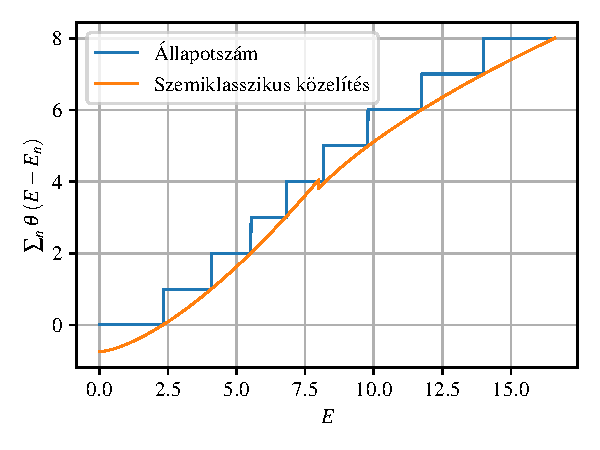
\includegraphics[scale=1]{./figs/allapotszam.pdf}
	\caption[Szemiklasszikus állapotszám]{A szemiklasszikus és egzakt energiaszintek összevetése. A kék vonal az egzakt energiák által meghatározott állapotszám. A narancssárga vonal pedig \aeqref{semiclassicallevels:e1} és \aeqref{semiclassicallevels:e2} egyenletekből kifejezett $n$ az energia függvényében, $E$ és $FL$ relációjának megfelelően.}
	\label{semiclassicallevels:allapotszam}
\end{figure}
\begin{figure}[H]
	\centering
	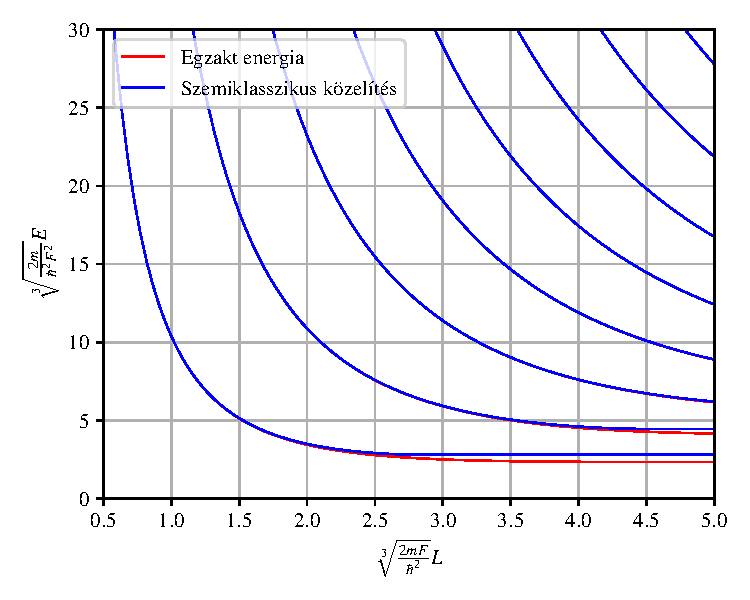
\includegraphics[scale=1]{./figs/energiaszintkozelites.pdf}
	\caption[Szemiklasszikus energiaszintek]{Az ábra a szemiklasszikus energiaszinteket hasonlítja össze az egzakt energiaszintekkel. Ez az ábra is a $bE$ és $aL$ közötti relációt ábrázolja. A szemiklasszikus közelítés nagy kvantumszámok illetve $E \gg FL$ esetén pontos. Utóbbi oka, hogy ebben az esetben a potenciál elhanyagolható, és a potenciál nélküli végtelen potenciálgödör energiaszintjeit pedig a szemiklasszikus közelítés egzaktul megadja.}
	\label{semiclassicallevels:kozelites}
\end{figure}
\begin{figure}[H]
	\centering
	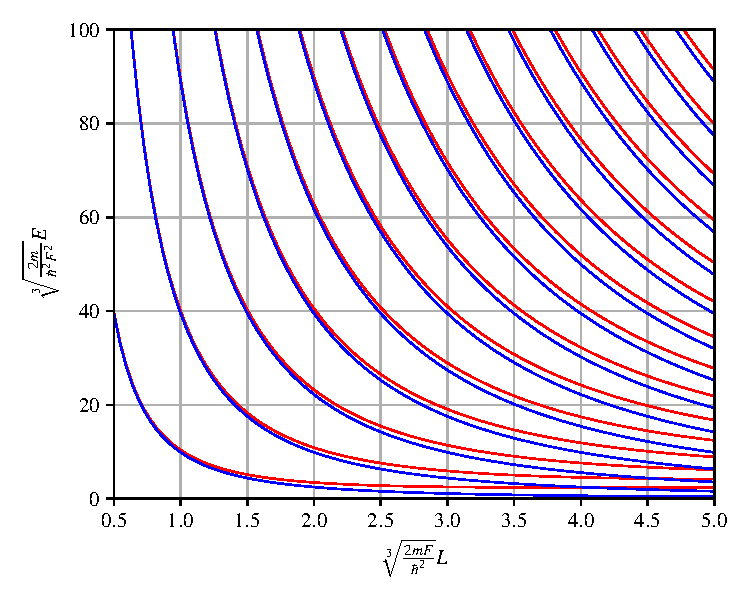
\includegraphics[scale=1]{./figs/infsquareenergia.pdf}
	\caption[Végtelen potenciálgödör energiaszintjei]{Az ábrán a végtelen potenciálgödör és az egzakt energiaszintek összehasonlítása látható. Ez csak az $E \gg FL$ esetben jó közelítés, a szemiklasszikus energiaszintek jóval pontosabbak.}
	\label{semiclassicallevels:squarewell}
\end{figure}